\section{Identification}
\label{sec:identification}
\subsection{Segmentation}

\todo[inline,color=red]{Identification - Segmentation}

Why won't projection segmentation work for us? Want to be able to isolate stems and beams, projection segmentation only gives vertical sections


\subsection{Feature Extraction}

\subsubsection{Downsampling}

\todo[inline,color=red]{Techniques - Feature Extraction: Downsampling}

\subsubsection{Statistical Properties}
\label{sec:statistical-properties}

\todo[inline,color=red]{Techniques - Feature Extraction: Stats Properties}

Moments, Centroids, Height etc

\subsubsection{Run Length Encoding}\label{sec:identification-rle}
To improve the speed of my application, I utilised \acrfull{RLE} (covered in \cref{sec:tb-rle}) to improve storage and retrieval times during feature extraction and classification by up to 97\% (\cref{table:rle-improvement}).

\begin{table}[h]

    \begin{tabularx}{\textwidth}{ X X X X }
    \toprule
    Metric                  & Without RLE   & With RLE   & Improvement \\
    \midrule
    Storage Required        & 759 MB        & 22 MB      & 91.7\%      \\
    Total Retrieval Time    & 1639 ms       & 42 ms      & 97.4\% \\
    \bottomrule
    \end{tabularx}

    \label{table:rle-improvement}
    \caption{Improvements after implementing RLE, tested on a sample set of 3000 components}
\end{table}

\subsection{Classification}
\label{sec:implementation-classification}

Classifiers are created by taking a sets of previously labelled samples and building a model which attempts to provide the most accurate relation between the samples and their labels. This allows new samples to be classified using the model to apply the most likely (and hopefully correct) label.

In order to maximise the accuracy of my classifications, I ran multiple experiments on different classifiers before deciding on which one I would apply in my application.

\subsubsection{K Nearest Neighbour}

For the K Nearest Neighbour algorithm, I tried two different feature vectors, the first was using the statistical properties outlined in \cref{sec:statistical-properties} and the second was a downsampled binary image flattened into a 1D array. 

An initial attempt at classification using statistical properties and a KNN classifier wasn't all that successful as you can see from the confusion matrix and accuracy scores in \cref{fig:knn-stats}. Most components were incorrectly classified as crotchet heads though I was unable to come up with a good explanation as to why and it's something which it would be interesting to investigate further in future.

\begin{figure}
  \centering
  \begin{subtable}[b]{\linewidth}
    \tiny
    \begin{tabularx}{\textwidth}{r|XXXXXXXXXXXXXXXXXXXXXX}
         & \rot{crotchetrest}  & \rot{minimhead}  & \rot{note\_complex}  & \rot{bassclef}  & \rot{beam\_complex}  & \rot{sharp}  & \rot{semibreve}  & \rot{quaverrest}  & \rot{barline}  & \rot{quavertaildown}  & \rot{minimsemibreverest}  & \rot{flat}  & \rot{crotchethead}  & \rot{stem}  & \rot{trebleclef}  & \rot{digit\_8}  & \rot{natural}  & \rot{digit\_3}  & \rot{digit\_2}  & \rot{digit\_4}  & \rot{quavertailup}  & \rot{dot} \\
      \midrule
    crotchetrest & 0 & 0 & 0 & 0 & 0 & 0 & 0 & 0 & 0 & 0 & 0 & 0 & 44 & 0 & 0 & 0 & 0 & 0 & 0 & 0 & 0 & 0 \\
    minimhead & 0 & 16 & 0 & 0 & 0 & 0 & 0 & 0 & 0 & 0 & 0 & 0 & 48 & 0 & 0 & 0 & 0 & 0 & 0 & 0 & 0 & 0 \\
    note\_complex & 0 & 0 & 32 & 0 & 0 & 0 & 0 & 0 & 0 & 0 & 0 & 0 & 87 & 0 & 0 & 0 & 0 & 0 & 0 & 0 & 0 & 0 \\
    bassclef & 0 & 0 & 0 & 0 & 0 & 0 & 0 & 0 & 0 & 0 & 0 & 0 & 37 & 0 & 0 & 0 & 0 & 0 & 0 & 0 & 0 & 0 \\
    beam\_complex & 0 & 0 & 0 & 0 & 0 & 0 & 0 & 0 & 0 & 0 & 0 & 0 & 1 & 0 & 0 & 0 & 0 & 0 & 0 & 0 & 0 & 0 \\
    sharp & 0 & 0 & 0 & 0 & 0 & 6 & 0 & 0 & 0 & 0 & 0 & 0 & 46 & 0 & 0 & 0 & 0 & 0 & 0 & 0 & 0 & 0 \\
    semibreve & 0 & 0 & 0 & 0 & 0 & 0 & 1 & 0 & 0 & 0 & 0 & 0 & 37 & 0 & 0 & 0 & 0 & 0 & 0 & 0 & 0 & 0 \\
    quaverrest & 0 & 0 & 0 & 0 & 0 & 0 & 0 & 0 & 0 & 0 & 0 & 0 & 36 & 0 & 0 & 0 & 0 & 0 & 0 & 0 & 0 & 0 \\
    barline & 0 & 0 & 0 & 0 & 0 & 0 & 0 & 0 & 0 & 0 & 0 & 0 & 32 & 0 & 0 & 0 & 0 & 0 & 0 & 0 & 0 & 0 \\
    quavertaildown & 0 & 0 & 0 & 0 & 0 & 0 & 0 & 0 & 0 & 0 & 0 & 0 & 10 & 0 & 0 & 0 & 0 & 0 & 0 & 0 & 0 & 0 \\
    minimsemibreverest & 0 & 0 & 0 & 0 & 0 & 0 & 0 & 0 & 0 & 0 & 1 & 0 & 9 & 0 & 0 & 0 & 0 & 0 & 0 & 0 & 0 & 0 \\
    flat & 0 & 0 & 0 & 0 & 0 & 0 & 0 & 0 & 0 & 0 & 0 & 2 & 50 & 0 & 0 & 0 & 0 & 0 & 0 & 0 & 0 & 0 \\
    crotchethead & 0 & 0 & 0 & 0 & 0 & 0 & 0 & 0 & 0 & 0 & 0 & 0 & 133 & 0 & 0 & 0 & 0 & 0 & 0 & 0 & 0 & 0 \\
    stem & 0 & 0 & 0 & 0 & 0 & 0 & 0 & 0 & 0 & 0 & 0 & 0 & 60 & 24 & 0 & 0 & 0 & 0 & 0 & 0 & 0 & 0 \\
    trebleclef & 0 & 0 & 0 & 0 & 0 & 0 & 0 & 0 & 0 & 0 & 0 & 0 & 40 & 0 & 2 & 0 & 0 & 0 & 0 & 0 & 0 & 0 \\
    digit\_8 & 0 & 0 & 0 & 0 & 0 & 0 & 0 & 0 & 0 & 0 & 0 & 0 & 0 & 0 & 0 & 1 & 0 & 0 & 0 & 0 & 0 & 0 \\
    natural & 0 & 0 & 0 & 0 & 0 & 0 & 0 & 0 & 0 & 0 & 0 & 0 & 37 & 0 & 0 & 0 & 0 & 0 & 0 & 0 & 0 & 0 \\
    digit\_3 & 0 & 0 & 0 & 0 & 0 & 0 & 0 & 0 & 0 & 0 & 0 & 0 & 7 & 0 & 0 & 0 & 0 & 2 & 0 & 0 & 0 & 0 \\
    digit\_2 & 0 & 0 & 0 & 0 & 0 & 0 & 0 & 0 & 0 & 0 & 0 & 0 & 9 & 0 & 0 & 0 & 0 & 0 & 0 & 0 & 0 & 0 \\
    digit\_4 & 0 & 0 & 0 & 0 & 0 & 0 & 0 & 0 & 0 & 0 & 0 & 0 & 19 & 0 & 0 & 0 & 0 & 0 & 0 & 7 & 0 & 0 \\
    quavertailup & 0 & 0 & 0 & 0 & 0 & 0 & 0 & 0 & 0 & 0 & 0 & 0 & 11 & 0 & 0 & 0 & 0 & 0 & 0 & 0 & 3 & 0 \\
    dot & 0 & 0 & 0 & 0 & 0 & 0 & 0 & 0 & 0 & 0 & 0 & 0 & 27 & 0 & 0 & 0 & 0 & 0 & 0 & 0 & 0 & 15 \\
    \end{tabularx}
  \end{subtable}

  \vspace{0.8cm}

  \begin{subtable}[b]{.4\linewidth}
    \begin{tabularx}{\linewidth}{lll}
      \toprule
      Accuracy & Precision & Recall \\
      \midrule
      0.275 & 0.645 & 0.275 \\
      \bottomrule
    \end{tabularx}
  \end{subtable}
  
  \caption{KNN classifier results using statistical features}
  \label{fig:knn-stats}
\end{figure}

For the downsampled image features, I ran a series of trials for different dimensions from 10px to 100px in both width and height (in 10px increments), averaging 3 repeats per dimension (each with a different training/testing split) and then generating a matrix of scores (which can be seen in full in \cref{table:height-width-matrix}).

Since most objects on a stave have a more vertical aspect ratio, I first graphed the average and maximum of the scores for each different height across all widths to see if there were any trends such as taller images producing higher accuracy.

The results can be seen in \cref{fig:height-downsample} and it seemed that in general, very short images ($\leq 20\text{px}$) gave worse results than tall ones but there wasn't anything conclusive and the gains from very tall images as opposed to fairly small images were minimal. Since there wasn't a height which clearly stood out, an analysis of the full matrix was done to find the highest scoring height and width combinations.

The top ten experimental accuracies from the tested dimensions are listed in \cref{table:knn-width-height-top} and I eventually selected $20\times50\text{px}$ as my downsampled dimension, the reason being that although larger dimensions did technically produce better accuracies, they were only \emph{slightly} better and would have resulted in many more pixels in the feature vector, slowing down the process of building a classifier and testing samples.

\begin{figure}[H]
  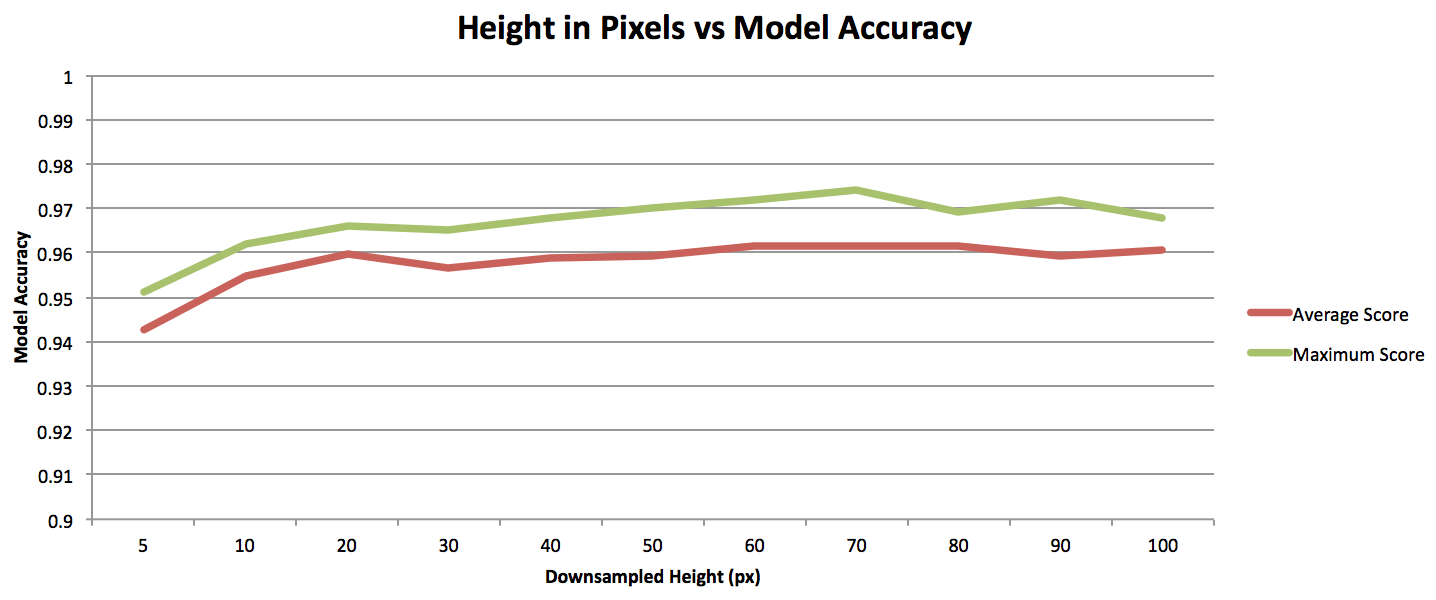
\includegraphics[width=\linewidth]{gfx/techniques/downsampling-height-vs-accuracy.png}
  \caption{The effect of downsampled image height on accuracy}
  \label{fig:height-downsample}
\end{figure}

\begin{table}[H]

    \begin{tabularx}{\textwidth}{ r X X X X }
    \toprule
    & Width & Height & Total Pixels & Accuracy \\
    \midrule
    & 50  & 70  & 3500 & 0.974 \\
    & 20  & 60  & 1200 & 0.971 \\
    & 20  & 70  & 1400 & 0.97 \\
    $\rightarrow$ & \textbf{20}  & \textbf{50}  & \textbf{1000} & \textbf{0.969} \\
    & 30  & 70  & 2100 & 0.969 \\
    & 100 & 70  & 7000 & 0.969 \\
    & 20  & 40  & 800  & 0.968 \\
    & 70  & 50  & 3500 & 0.967 \\
    & 60  & 60  & 3600 & 0.967 \\
    & 20  & 100 & 2000 & 0.967 \\
    \bottomrule
    \end{tabularx}

    \label{table:knn-width-height-top}
    \caption{Top 10 accuracy scores for different width and height combinations, the selection dimensions used in the classifier are highlighted and the full results can be found in \cref{table:height-width-matrix}}
\end{table}

Initial results on attempting to distinguish between all components were positive and I was able to achieve around 93\% accuracy as seen in \cref{table:confusion-matrix-knn-img-all}.

\begin{figure}[H]
  \centering
  \begin{subtable}[b]{\linewidth}
    \small
    \begin{tabularx}{\textwidth}{r|XXXXXXXXXXXXXXXXXXXXX}
         & \rot{flat}  & \rot{trebleclef}  & \rot{crotchetrest}  & \rot{digit\_8}  & \rot{minimhead}  & \rot{crotchethead}  & \rot{digit\_2}  & \rot{digit\_4}  & \rot{quaverrest}  & \rot{semibreve}  & \rot{beam\_complex}  & \rot{quavertailup}  & \rot{bassclef}  & \rot{sharp}  & \rot{digit\_3}  & \rot{natural}  & \rot{barline}  & \rot{stem}  & \rot{quavertaildown}  & \rot{dot}  & \rot{minimsemibreverest} \\
      \midrule
    flat & 62 & 0 & 0 & 0 & 0 & 0 & 0 & 0 & 0 & 0 & 0 & 0 & 0 & 0 & 0 & 0 & 0 & 0 & 0 & 0 & 0 \\
    trebleclef & 0 & 53 & 0 & 0 & 0 & 0 & 0 & 0 & 0 & 0 & 0 & 0 & 0 & 0 & 0 & 0 & 0 & 0 & 0 & 0 & 0 \\
    crotchetrest & 0 & 0 & 37 & 0 & 0 & 0 & 0 & 0 & 0 & 0 & 0 & 0 & 0 & 0 & 0 & 0 & 0 & 0 & 0 & 0 & 0 \\
    digit\_8 & 0 & 0 & 0 & 0 & 0 & 0 & 0 & 0 & 0 & 0 & 0 & 0 & 0 & 0 & 0 & 0 & 0 & 0 & 0 & 0 & 0 \\
    minimhead & 0 & 0 & 0 & 0 & 43 & 0 & 0 & 0 & 0 & 3 & 0 & 0 & 0 & 0 & 0 & 0 & 0 & 0 & 0 & 0 & 0 \\
    crotchethead & 0 & 0 & 0 & 0 & 0 & 98 & 0 & 0 & 0 & 0 & 0 & 0 & 0 & 0 & 0 & 0 & 0 & 0 & 0 & 0 & 0 \\
    digit\_2 & 0 & 0 & 0 & 0 & 0 & 0 & 16 & 0 & 0 & 0 & 0 & 0 & 0 & 0 & 0 & 0 & 0 & 0 & 0 & 0 & 0 \\
    digit\_4 & 0 & 0 & 0 & 0 & 0 & 0 & 0 & 28 & 0 & 0 & 0 & 0 & 0 & 0 & 0 & 0 & 0 & 0 & 0 & 0 & 0 \\
    quaverrest & 0 & 0 & 0 & 0 & 0 & 0 & 0 & 0 & 35 & 0 & 0 & 0 & 0 & 0 & 0 & 0 & 0 & 0 & 0 & 0 & 0 \\
    semibreve & 0 & 0 & 0 & 0 & 0 & 0 & 0 & 0 & 0 & 37 & 0 & 0 & 0 & 0 & 0 & 0 & 0 & 0 & 0 & 0 & 0 \\
    beam\_complex & 0 & 1 & 0 & 0 & 0 & 0 & 0 & 0 & 0 & 0 & 0 & 0 & 0 & 0 & 0 & 0 & 0 & 0 & 0 & 0 & 0 \\
    quavertailup & 0 & 0 & 1 & 0 & 0 & 0 & 0 & 0 & 0 & 0 & 0 & 17 & 0 & 0 & 0 & 0 & 0 & 0 & 0 & 0 & 0 \\
    bassclef & 0 & 0 & 0 & 0 & 0 & 0 & 0 & 0 & 0 & 0 & 0 & 0 & 35 & 0 & 0 & 0 & 0 & 0 & 0 & 0 & 0 \\
    sharp & 0 & 0 & 0 & 0 & 0 & 0 & 0 & 0 & 0 & 0 & 0 & 0 & 0 & 55 & 0 & 0 & 0 & 0 & 0 & 0 & 0 \\
    digit\_3 & 0 & 0 & 0 & 0 & 0 & 0 & 0 & 0 & 0 & 0 & 0 & 0 & 0 & 0 & 5 & 0 & 0 & 0 & 0 & 0 & 0 \\
    natural & 0 & 0 & 0 & 0 & 0 & 0 & 0 & 0 & 0 & 0 & 0 & 0 & 0 & 0 & 0 & 49 & 0 & 0 & 0 & 0 & 0 \\
    barline & 1 & 0 & 0 & 0 & 0 & 0 & 0 & 0 & 0 & 0 & 0 & 0 & 0 & 0 & 0 & 0 & 20 & 18 & 0 & 0 & 0 \\
    stem & 0 & 5 & 0 & 0 & 0 & 0 & 0 & 0 & 0 & 0 & 0 & 0 & 0 & 0 & 0 & 0 & 3 & 92 & 0 & 0 & 0 \\
    quavertaildown & 0 & 0 & 0 & 0 & 0 & 0 & 0 & 0 & 0 & 0 & 0 & 0 & 0 & 0 & 0 & 0 & 0 & 0 & 9 & 0 & 0 \\
    dot & 0 & 0 & 0 & 0 & 0 & 7 & 0 & 0 & 0 & 0 & 0 & 0 & 0 & 0 & 0 & 0 & 0 & 2 & 0 & 38 & 0 \\
    minimsemibreverest & 0 & 0 & 0 & 0 & 0 & 0 & 0 & 0 & 0 & 0 & 0 & 0 & 0 & 0 & 0 & 0 & 0 & 6 & 0 & 5 & 0 \\
    \end{tabularx}
  \end{subtable}
  \vspace{0.8cm}
  \begin{subtable}[b]{.4\linewidth}
    \begin{tabularx}{\linewidth}{lll}
      \toprule
      Accuracy & Precision & Recall \\
      \midrule
      0.933 & 0.922 & 0.933 \\
      \bottomrule
    \end{tabularx}
  \end{subtable}
  \caption{Accuracy achieved using a KNN classifier trained on downsampled 20x50px images}
  \label{table:confusion-matrix-knn-img-all}
\end{figure}

We can see that a few components in \cref{table:confusion-matrix-knn-img-all} are confused more than others, for example \emph{stems} and \emph{barlines}. To mitigate this, we can employ the use of hierarchical classification. Instead of trying to classify every single component at once, we can instead perform an initial `high level' classification, followed by further secondary classifications. The best example of this is a note. Instead of trying to separate a note straight away into heads stems and beams, it's sufficient to simply classify it as a `note\_complex' entity and perform more detailed classification of components later.

Using a two-stage classifier much more satisfactory results were achieved, with an initial classification accuracy of 98.5\% (\cref{fig:knn-level1}) and a secondary classification accuracy of 100\% (\cref{fig:knn-level2})!

\begin{figure}[H]
  \centering
  
  \vspace{0.4cm}
  
  \begin{subtable}[b]{\linewidth}
    \centering
    \small
    \begin{tabularx}{.8\textwidth}{r|XXXXXXXXXXXXXXXXX}
         & \rot{flat}  & \rot{digit\_4}  & \rot{trebleclef}  & \rot{crotchetrest}  & \rot{digit\_8}  & \rot{dot}  & \rot{digit\_3}  & \rot{digit\_2}  & \rot{semibreve}  & \rot{quaverrest}  & \rot{note\_complex}  & \rot{natural}  & \rot{bassclef}  & \rot{beam\_complex}  & \rot{sharp}  & \rot{barline}  & \rot{minimsemibreverest} \\
      \midrule
    flat & 55 & 0 & 0 & 0 & 0 & 0 & 0 & 0 & 0 & 0 & 0 & 0 & 0 & 0 & 0 & 0 & 0 \\
    digit\_4 & 0 & 24 & 0 & 0 & 0 & 0 & 0 & 0 & 0 & 0 & 0 & 0 & 0 & 0 & 0 & 0 & 0 \\
    trebleclef & 0 & 0 & 49 & 0 & 0 & 0 & 0 & 0 & 0 & 0 & 0 & 0 & 0 & 0 & 0 & 0 & 0 \\
    crotchetrest & 0 & 0 & 0 & 35 & 0 & 0 & 0 & 0 & 0 & 0 & 0 & 0 & 0 & 0 & 0 & 0 & 0 \\
    digit\_8 & 0 & 0 & 0 & 0 & 0 & 0 & 0 & 0 & 0 & 0 & 0 & 0 & 0 & 0 & 0 & 0 & 0 \\
    dot & 0 & 0 & 0 & 0 & 0 & 45 & 0 & 0 & 0 & 0 & 0 & 0 & 0 & 0 & 0 & 0 & 0 \\
    digit\_3 & 0 & 0 & 0 & 2 & 0 & 0 & 3 & 0 & 0 & 0 & 0 & 0 & 0 & 0 & 0 & 0 & 0 \\
    digit\_2 & 0 & 0 & 0 & 0 & 0 & 0 & 0 & 16 & 0 & 0 & 0 & 0 & 0 & 0 & 0 & 0 & 0 \\
    semibreve & 0 & 0 & 0 & 0 & 0 & 0 & 0 & 0 & 47 & 0 & 0 & 0 & 0 & 0 & 0 & 0 & 0 \\
    quaverrest & 0 & 0 & 0 & 0 & 0 & 0 & 0 & 0 & 0 & 35 & 0 & 0 & 0 & 0 & 0 & 0 & 0 \\
    note\_complex & 0 & 0 & 0 & 0 & 0 & 0 & 0 & 0 & 0 & 0 & 125 & 0 & 2 & 0 & 0 & 0 & 0 \\
    natural & 0 & 0 & 0 & 0 & 0 & 0 & 0 & 0 & 0 & 0 & 0 & 35 & 0 & 0 & 0 & 0 & 0 \\
    bassclef & 0 & 0 & 0 & 0 & 0 & 0 & 0 & 0 & 0 & 0 & 0 & 0 & 34 & 0 & 0 & 0 & 0 \\
    beam\_complex & 0 & 0 & 0 & 0 & 0 & 0 & 0 & 0 & 0 & 0 & 0 & 0 & 0 & 0 & 0 & 0 & 0 \\
    sharp & 0 & 2 & 0 & 0 & 0 & 0 & 0 & 0 & 0 & 0 & 0 & 0 & 0 & 0 & 60 & 0 & 0 \\
    barline & 0 & 0 & 0 & 0 & 0 & 0 & 0 & 0 & 0 & 0 & 0 & 0 & 0 & 0 & 0 & 27 & 0 \\
    minimsemibreverest & 0 & 0 & 0 & 0 & 0 & 3 & 0 & 0 & 0 & 0 & 0 & 0 & 0 & 0 & 0 & 0 & 3 \\
    \end{tabularx}
  \end{subtable}
  
  \vspace{0.8cm}
  
  \begin{subtable}[b]{.4\linewidth}
    \begin{tabularx}{\linewidth}{lll}
      \toprule
      Accuracy & Precision & Recall \\
      \midrule
      0.985 & 0.986 & 0.985 \\
      \bottomrule
    \end{tabularx}
  \end{subtable}
  
  \vspace{0.4cm}
  
  \caption{1st level KNN Classifier Results}
  \label{fig:knn-level1}
\end{figure}

\begin{figure}[H]
  \centering
  
  \vspace{0.4cm}
  
  \begin{subtable}[b]{.4\linewidth}
    \begin{tabularx}{\textwidth}{r|XXXXX}
         & \rot{minimhead}  & \rot{crotchethead}  & \rot{quavertailup}  & \rot{quavertaildown}  & \rot{stem} \\
      \midrule
    minimhead & 51 & 0 & 0 & 0 & 0 \\
    crotchethead & 0 & 118 & 0 & 0 & 0 \\
    quavertailup & 0 & 0 & 23 & 0 & 0 \\
    quavertaildown & 0 & 0 & 0 & 5 & 0 \\
    stem & 0 & 0 & 0 & 0 & 93 \\
    \end{tabularx}
  \end{subtable}
  
  \vspace{0.8cm}
  
  \begin{subtable}[b]{.4\linewidth}
    \begin{tabularx}{\linewidth}{lll}
      \toprule
      Accuracy & Precision & Recall \\
      \midrule
      1.0 & 1.0 & 1.0 \\
      \bottomrule
    \end{tabularx}
  \end{subtable}
  
  \vspace{0.4cm}
  
  \caption{2nd level KNN Classifier Results}
  \label{fig:knn-level2}
\end{figure}


\subsubsection{Neural Net}

Although neural networks are also common in OMR, I was unfortunately unable to extract any great results from them during my experiments. The best classification result I got was by using Hierarchical Classification, where the network achieved an accuracy of 80.38\% for the 1st level classifier as seen in \cref{fig:nn-classification-data}. I used trained the network using Backwards Propogation and used two hidden sigmoidal layers of 25 nodes each.
As more potential classes were added, unfortunately the accuracy just decreased and so I chose to use KNN as my classification technique.

It should be noted, however, that since I didn't have the opportunity to study this material in class having not done any of the more advanced machine learning courses, it is quite possible that there were flaws in my implementation, indeed many people have great success using neural networks for this and similar applications, achieving high accuracy rates and it's something which is maybe worth coming back to again in future.

\begin{figure}[H]
  \centering
  
  \vspace{0.4cm}
  
  \begin{subtable}[b]{   \linewidth}
    \small
    \begin{tabularx}{\textwidth}{r|XXXXXXXXXXXXXXX}
    & \rot{crotchetrest} & \rot{semibreve} & \rot{dot} & \rot{flat} & \rot{digit\_2} & \rot{barline} & \rot{trebleclef} & \rot{sharp} & \rot{quaverrest} & \rot{digit\_3} & \rot{note\_complex} & \rot{natural} & \rot{digit\_4} & \rot{bassclef} & \rot{minimsemibreverest} \\
    \midrule
    crotchetrest       & 29 &  0 &  1 &  0  & 1 &  0 &  3 &  3 &  0 &  0 &   5  &  1  &  1  &  1  &  0 \\               
    semibreve          &  0 & 45 &  0 &  0  & 0 &  0 &  0 &  0 &  0 &  0 &   1  &  0  &  0  &  0  &  0 \\            
    dot                &  0 &  1 & 43 &  0  & 0 &  0 &  0 &  0 &  0 &  0 &   0  &  1  &  0  &  1  &  0 \\      
    flat               &  0 &  0 &  0 & 43  & 0 &  0 &  0 &  3 &  0 &  0 &   8  &  1  &  1  &  0  &  0 \\       
    digit\_2            &  0 &  0 &  1 &  0  & 5 &  0 &  0 &  0 &  0 &  0 &   4  &  0  &  0  &  0  &  0 \\          
    barline            &  0 &  0 & 10 &  0  & 0 & 28 &  2 &  1 &  0 &  0 &   0  &  0  &  2  &  0  &  0 \\          
    trebleclef         &  1 &  0 &  0 &  1  & 0 &  2 & 29 &  3 &  0 &  0 &   0  &  0  &  1  &  0  &  0 \\             
    sharp              &  1 &  0 &  2 &  0  & 0 &  1 &  1 & 46 &  0 &  0 &   0  &  0  &  1  &  0  &  0 \\        
    quaverrest         &  0 &  0 &  0 &  0  & 0 &  0 &  0 &  0 & 32 &  1 &   1  &  1  &  0  &  0  &  0 \\             
    digit\_3            &  0 &  0 &  0 &  0  & 0 &  0 &  2 &  1 &  0 &  0 &   3  &  0  &  0  &  0  &  0 \\          
    note\_complex       &  0 &  0 &  0 &  0  & 1 &  0 &  1 &  0 &  3 &  0 & 102  &  1  &  0  &  0  &  0 \\               
    natural            &  0 &  0 &  0 &  0  & 0 &  0 &  2 &  1 &  0 &  0 &   1  & 31  &  0  &  0  &  0 \\          
    digit\_4            &  1 &  1 &  0 &  0  & 0 &  2 &  3 &  4 &  0 &  0 &   4  &  0  & 10  &  0  &  0 \\          
    bassclef           &  0 &  0 &  0 &  0  & 0 &  0 &  0 &  0 &  1 &  0 &   4  &  0  &  0  & 28  &  0 \\           
    minimsemibreverest &  0 &  0 &  9 &  0  & 0 &  0 &  0 &  0 &  0 &  0 &   0  &  0  &  0  &  0  &  0 \\                    
    \end{tabularx}
  \end{subtable}
  
  \vspace{0.8cm}
  
  \begin{subtable}[b]{.4\linewidth}
    \begin{tabularx}{\linewidth}{lll}
      \toprule
      Accuracy & Precision & Recall \\
      \midrule
      0.804 & 0.797 & 0.804 \\
      \bottomrule
    \end{tabularx}
  \end{subtable}
  
  \vspace{0.4cm}
  
  \caption{1st level Neural Network Classifier Results}
  \label{fig:nn-classification-data}
\end{figure}


\subsection{Pitch}
\label{sec:pitch-identification}

For note heads and accidentals, it's important to know exactly where the centre of the note lies in order to correctly identify it's position on the stave. Doing this roughly is usually sufficient for OMR, however, since we would like to be able to feed back to the student if they aren't putting their notes in the right place \todo{Reference note position criteria} we need to be as accurate as possible.

Once the position has been determined, we can calculate the difference between that and the y coordinate of the various pitched components on the stave, assigning the pitch which is closest using \cref{alg:note-assignment}.

\begin{algorithm}[H]
\caption{Assigning a pitch to a component}
\label{alg:note-assignment}
\begin{algorithmic}[1]
\Procedure{GetNoteForComponent}{$component$}
    \State sum = \Call{GetComponentCentre}{$component$}
    \State min\_distance = $\infty$
    \State assigned\_pitch = None
    \For {each pitch in pitches}
      \State dist = \Call{ABS}{pitch\_coord - y}
      \If{dist $<$ min\_dist}
        \State min\_dist = dist
        \State allocated\_pitch = pitch
      \EndIf
	\EndFor
	\Return assigned\_pitch
\EndProcedure
\end{algorithmic}
\end{algorithm}

For a rough estimate of note head position, the simplest method is to simply use a known position such as $1/2$ or $1/3$ along the vertical axis and use that as an estimate for the centre. Indeed that's often what is done in traditional OMR. \todo{Reference for dividing in half to get centre}. \todo{I know one of the papers uses 1/3 for flats}. However we can get a more accurate position using alternative techniques as 


\subsubsection{Sharp Centres}
For the sharp centre, the centroid proved less than satisfactory it was easily affected by the length of the lines (see the blue centres in \cref{fig:sharp-centroids}), whereas in reality the `centre' of a sharp is determined by the position of it's island region in the middle.

By inverting the image and performing connected component segmentation, we can isolate the island region and after extracting the centroids from this region, we get a much more satisfactory identification of the sharp's centre, show in \cref{fig:sharp-centroids} by the intersecting red lines.

\begin{figure}[h!]
    \centering
    \begin{subfigure}[b]{.3\linewidth}
        \centering
        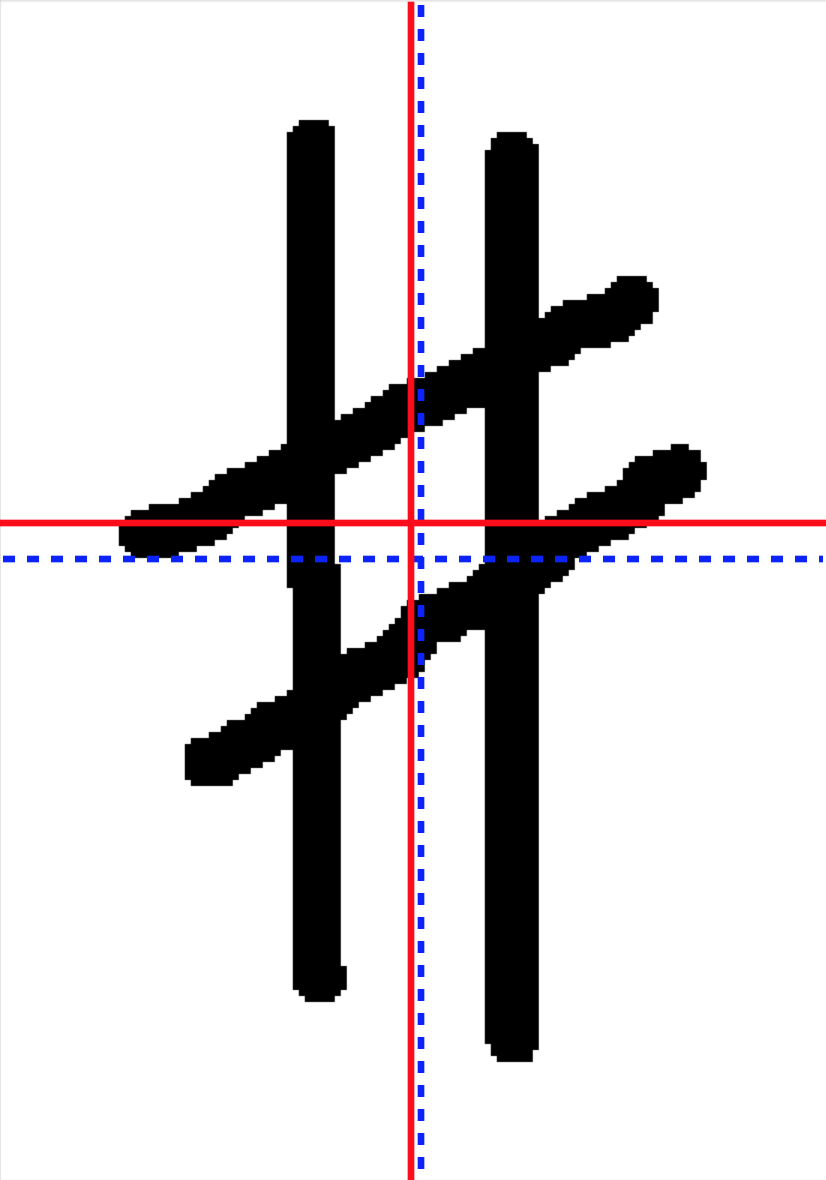
\includegraphics[height=5cm]{gfx/techniques/sharp-centroid-6109.png}
        \phantomsubcaption
    \end{subfigure}
    \begin{subfigure}[b]{.3\linewidth}
        \centering
        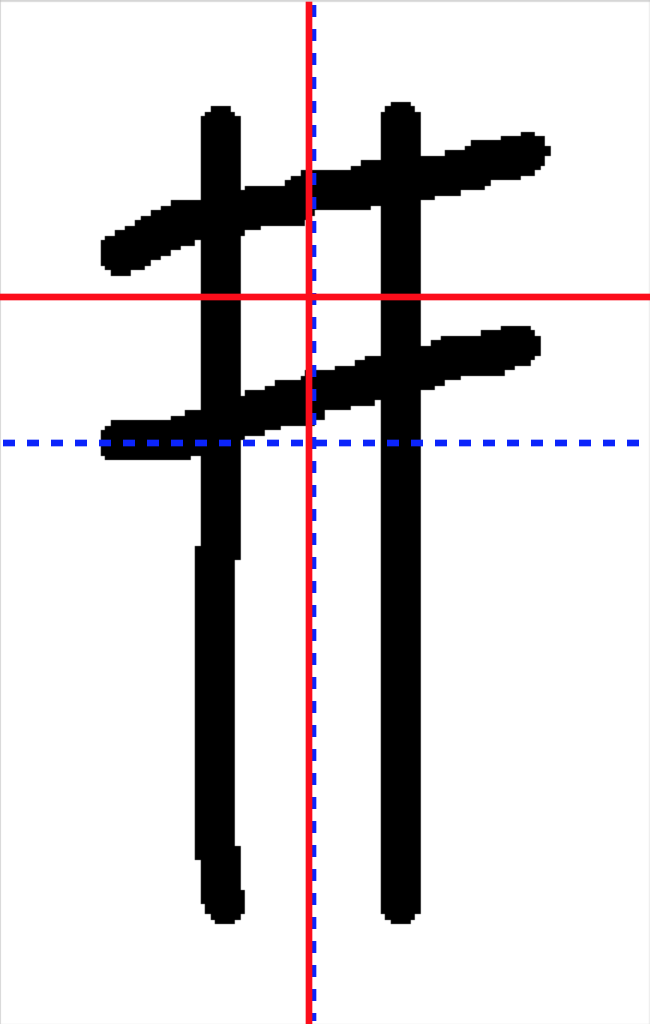
\includegraphics[height=5cm]{gfx/techniques/sharp-centroid-6110.png}
        \phantomsubcaption
    \end{subfigure}
    \begin{subfigure}[b]{.3\linewidth}
        \centering
        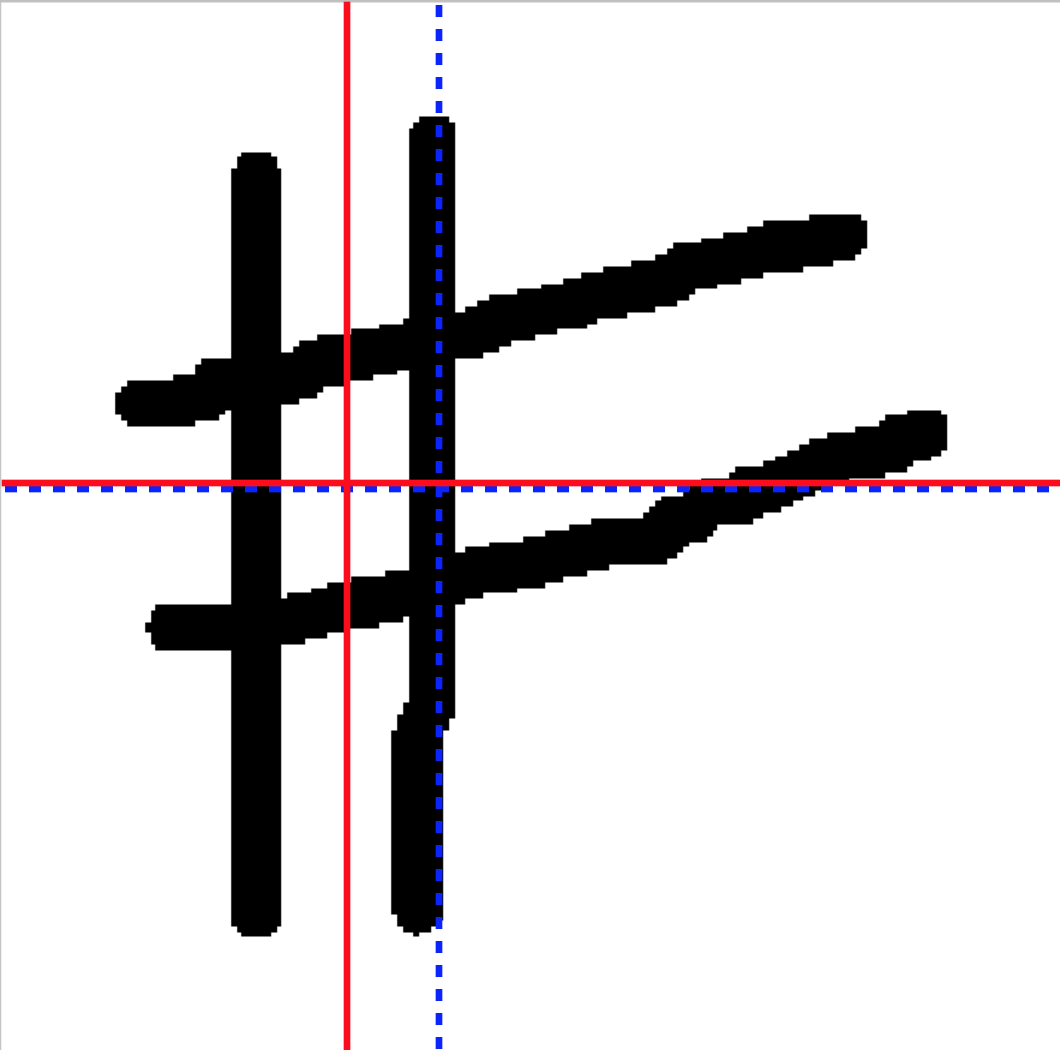
\includegraphics[height=5cm]{gfx/techniques/sharp-centroid-6108.png}
        \phantomsubcaption
    \end{subfigure}

  \caption{Identifying the true centres of the drawn sharps. Red intersecting lines show the true centres and blue intersecting lines show the centroid centres}
  \label{fig:sharp-centroids}
\end{figure}

\subsubsection{Flat Centres}

An unfortunate occurrence in flats during preliminary user testing was that of not joining the head up properly, an example of which can be seen in \cref{fig:flat-broken}. Ideally we would like to perform a similar technique to sharps, however we need some reliable way to compensate for potential breaks.

The first experiment I ran was to perform watershed segmentation by computing a distance transform on the flat, then by using the local maximum peaks as a starting point watershed segmentation was performed, resulting in the initial segmentation seen in \cref{fig:flat-broken-watershed}. From there, by merging neighbouring regions from smallest to largest, we can identify the `island' component (\cref{fig:flat-broken-merged}) and take the y coordinate of the centroid of this region.

\begin{figure}[H]
    \centering
    \begin{subfigure}[b]{.19\linewidth}
        \centering
        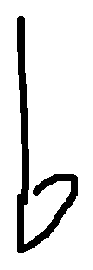
\includegraphics[height=5cm]{gfx/techniques/scoring/flats/6193-original.png}
        \caption{Original}
        \label{fig:flat-broken}
    \end{subfigure}
    \begin{subfigure}[b]{.19\linewidth}
        \centering
        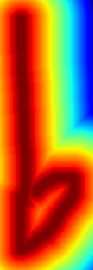
\includegraphics[height=5cm]{gfx/techniques/scoring/flats/6193-distance.png}
        \caption{Distance}
    \end{subfigure}
    \begin{subfigure}[b]{.19\linewidth}
        \centering
        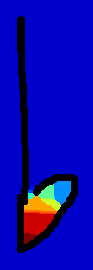
\includegraphics[height=5cm]{gfx/techniques/scoring/flats/6193-watershed.png}
        \caption{Watershed}
        \label{fig:flat-broken-watershed}
    \end{subfigure}
    \begin{subfigure}[b]{.19\linewidth}
        \centering
        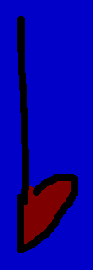
\includegraphics[height=5cm]{gfx/techniques/scoring/flats/6193-segmented.png}
        \caption{Merged}
        \label{fig:flat-broken-merged}
    \end{subfigure}
    \begin{subfigure}[b]{.19\linewidth}
        \centering
        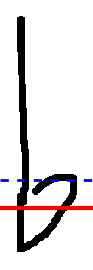
\includegraphics[height=5cm]{gfx/techniques/scoring/flats/6193-center.png}
        \caption{Centre}
    \end{subfigure}

  \caption{Identifying flat centre with watershed segmentation}
  \label{fig:flats-centre-watershed}
\end{figure}

An alternative solution uses dilations. This involves expanding the drawn image (and consequently shrinking the flat's `head' region) evenly until a distinct island region is formed (\cref{fig:flat-dilation}). Once that happens the vertical centre of the `head' can be established in the same way as outlined previously, using the centroid.

\begin{figure}[H]
    \centering
    \begin{subfigure}[b]{.2\linewidth}
        \centering
        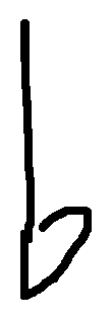
\includegraphics[height=5cm]{gfx/techniques/scoring/flats/6193-dilation-original.png}
        \caption{Original}
    \end{subfigure}
    \begin{subfigure}[b]{.2\linewidth}
        \centering
        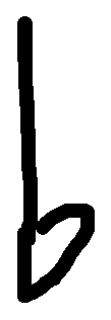
\includegraphics[height=5cm]{gfx/techniques/scoring/flats/6193-dilation-dilated.png}
        \caption{Dilation}
        \label{fig:flat-dilation}
    \end{subfigure}
    \begin{subfigure}[b]{.2\linewidth}
        \centering
        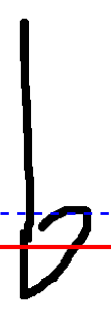
\includegraphics[height=5cm]{gfx/techniques/scoring/flats/6193-dilation-center}
        \caption{Centre}
    \end{subfigure}

  \caption{Identifying flat centre with dilation and connected component segmentation}
  \label{fig:flats-centre-dilation}
\end{figure}

\subsubsection{Note Head Centres}

For note heads, it was discovered that the centroid was a good representation of the centre, even in case of broken minims as seen in \cref{fig:broken-minim}

\begin{figure}[H]
    \centering
    \begin{subfigure}[b]{.32\linewidth}
        \centering
        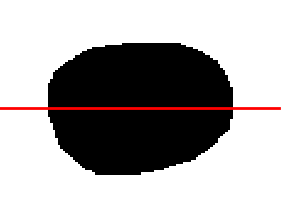
\includegraphics[width=\linewidth]{gfx/techniques/scoring/note-head/1906-centroid-centre.png}
        \caption{Crotchet Head}
    \end{subfigure}
    \begin{subfigure}[b]{.32\linewidth}
        \centering
        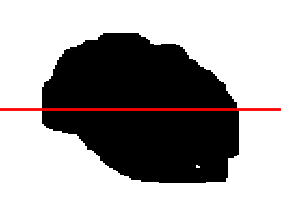
\includegraphics[width=\linewidth]{gfx/techniques/scoring/note-head/6189-centroid-centre.png}
        \caption{Wonky Crotchet Head}
    \end{subfigure}
    \begin{subfigure}[b]{.32\linewidth}
        \centering
        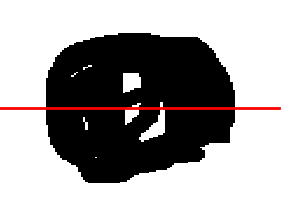
\includegraphics[width=\linewidth]{gfx/techniques/scoring/note-head/6192-centroid-centre.png}
        \caption{Inconsistent Crotchet Head}
    \end{subfigure}
    
    \begin{subfigure}[b]{.3\linewidth}
        \centering
        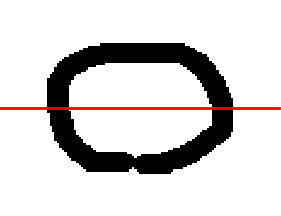
\includegraphics[width=\linewidth]{gfx/techniques/scoring/note-head/1818-centroid-centre.png}
        \caption{Minim Head}
    \end{subfigure}
    \begin{subfigure}[b]{.3\linewidth}
        \centering
        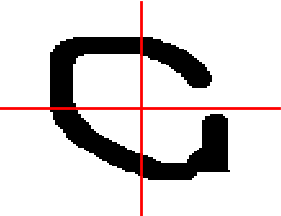
\includegraphics[width=\linewidth]{gfx/techniques/scoring/note-head/6105-centroid-centre.png}
        \caption{Broken Minim Head}
    \end{subfigure}

  \caption{Filled and hollow note heads with their centres identified by two red intersecting lines}
  \label{fig:ccl-two-pass}
\end{figure}

\subsection{Duration}
\label{sec:duration-identification}

There are two main steps to the process for calculating note duration. The first is the extraction of the fundamental note value, is it a semibreve, minim, crotchet, quaver or semiquaver? For a  semibreve, the note value will always be four, however for other notes, things are not so straightforward.

We first examine each note individually to ascertain it's the components of which it is comprised and assign it note a base value. For example we are particularly interested in the note head (is it solid or hollow) and any tails or beaming. An outline of this heuristic can be seen in \cref{fig:note-duration-flow-chart}.

The number of tails is fairly straightforward as they are attached to isolate notes, in a complex beam such as that in \cref{fig:complex-beam-stablish} however, we need to have some way to work out which notes have which values. To do this, a section the width of $\text{Stave Space} / 2$ is examined either side of the note's stem \todo{How did/do we handle angled stems here?}. The beam is analysed in these segments for the maximum number of vertical black runs which represents the number beams.

\begin{figure}[H]
  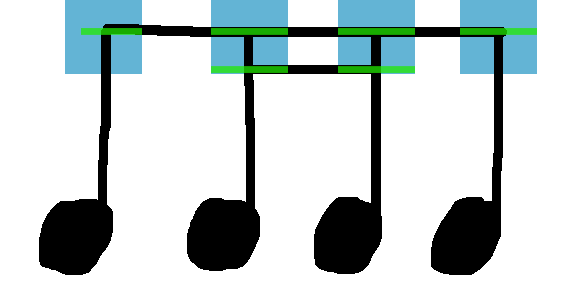
\includegraphics[width=\linewidth]{gfx/implementation/beam-identification.png}
  \caption{Calculating the number of beams to get note values. Blue areas show the regions scanned and green lines represent the maximum count of vertical black runs found}
  \label{fig:complex-beam-establish}
\end{figure}

\begin{figure}[H]
  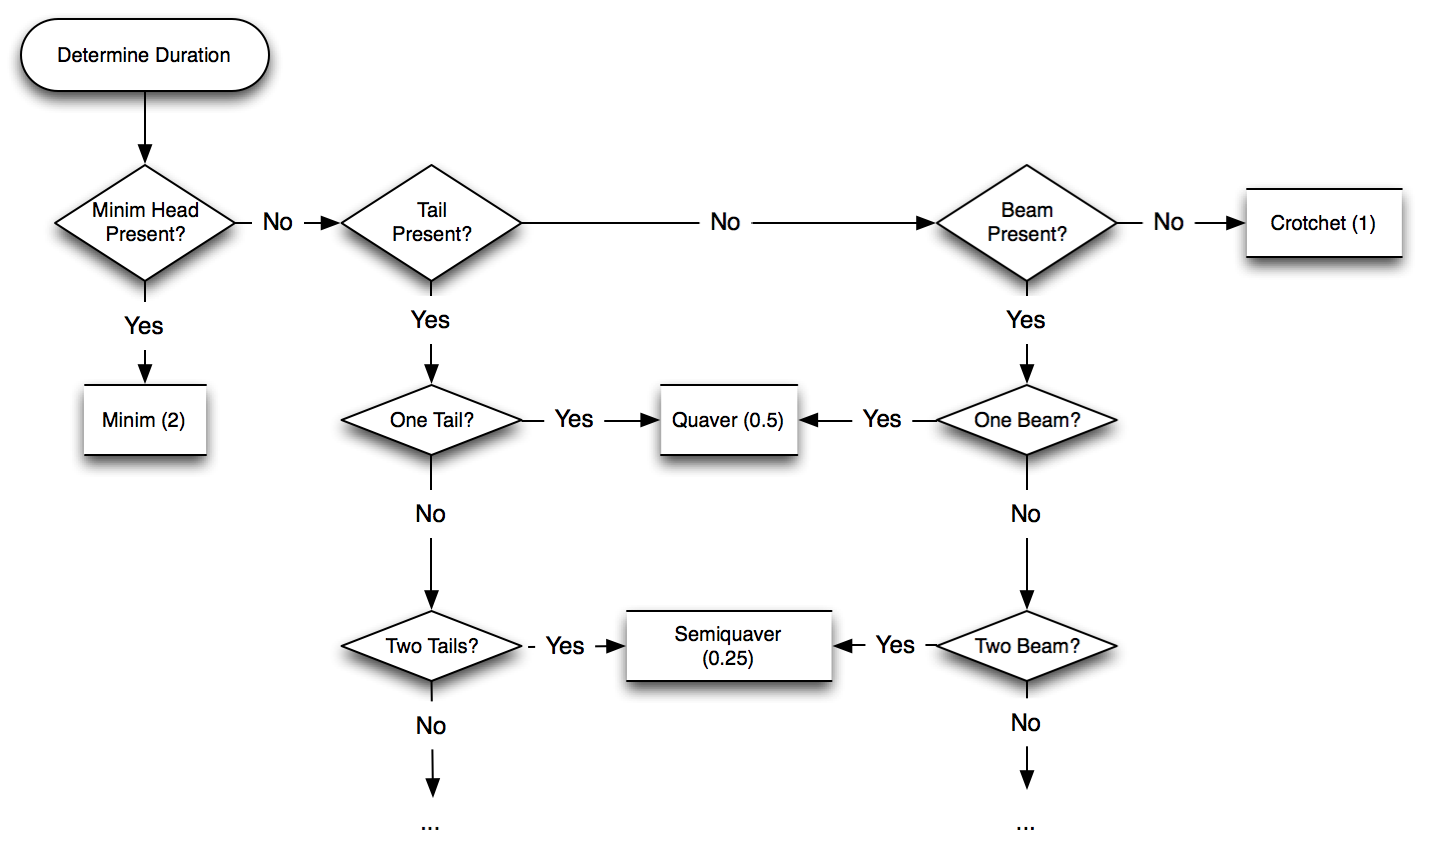
\includegraphics[width=\linewidth]{gfx/implementation/duration-diagram.png}
  \caption{Flow chart for establishing base note duration}
  \label{fig:note-duration-flow-chart}
\end{figure}

Note that with regards to tails and beaming, since every additional beam or tail present for the note divides it's value by two (examples can be seen in \todo{reference note lengths from background}) we can generalise this section of the heuristic to deal with any number of beams and tails.

Once the base value has been obtained, we perform a final check of the area surrounding the note centre for any `modifier' dots. These extend the duration of the note by half, so for example, a dotted crotchet would last 1.5 beats as opposed to 1 beat without the dot. The region searched equates to half a staff space down and either side of the note as shown in \cref{fig:identify-dot}, anything outside of this region is ignored.


\begin{figure}[H]
  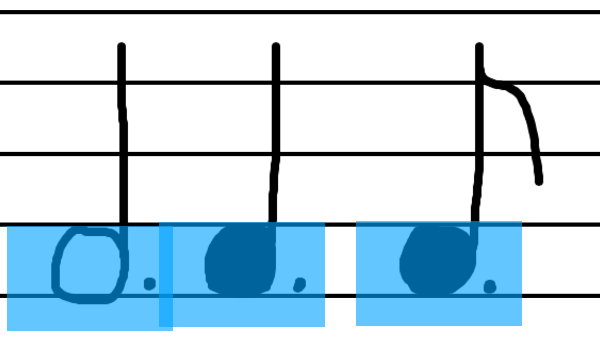
\includegraphics[width=\linewidth]{gfx/implementation/dot-identification.png}
  \caption{Searching for dots which would modify a note's length. Blue areas are the searched space for each note}
  \label{fig:identify-dot}
\end{figure}